% *********************************************************************
% © 2021–2026 Jeremy Sylvestre
%
% Permission is granted to copy, distribute and/or modify this document
% under the terms of the GNU Free Documentation License, Version 1.3 or
% any later version published by the Free Software Foundation; with no
% Invariant Sections, no Front-Cover Texts, and no Back-Cover Texts. A
% copy of the license is included in the appendix entitled “GNU Free
% Documentation License” that appears in the output document of this
% PreTeXt source code. All trademarks™ are the registered® marks of
% their respective owners.
%
% *********************************************************************

\newcommand*{\xmin}{-1}
\newcommand*{\xmax}{2.75}
\newcommand*{\ymin}{-8}
\newcommand*{\ymax}{17}

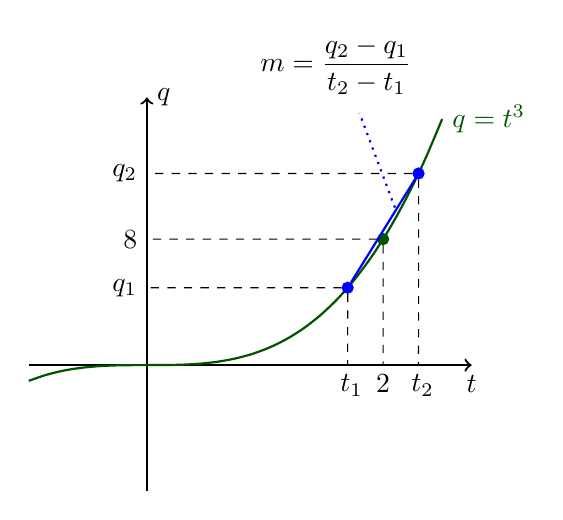
\begin{tikzpicture}
[
	closedpt/.style={circle,draw,fill,inner sep=0pt,minimum size=4pt},
	openpt/.style={circle,draw,inner sep=0pt,minimum size=4pt},
	yscale=0.2,xscale=1.5
]

	% axes
	\draw[->,thick] (\xmin,0) -- (\xmax,0) node[below] {$t$};
	\draw[->,thick] (0,\ymin) -- (0,\ymax) node[right] {$q$};

	\draw[green!33!black,thick,domain=-1:2.5,smooth] plot (\x,{\x * \x * \x}) node[right] {$q = t^3$};

	\node[closedpt,green!33!black] at (2,8) (pt) {};
	\node[closedpt,blue] at (1.7,4.913) (pt1) {};
	\node[closedpt,blue] at (2.3,12.167) (pt2) {};

	\draw[dashed] (pt) -- (2,0) node[below] {$2$};
	\draw[dashed] (pt) -- (0,8) node[left] {$8$};

	\draw[dashed] (pt1) -- (1.7,0) node[below,xshift=0.05cm] {$t_1$};
	\draw[dashed] (pt1) -- (0,4.913) node[left] {$q_1$};
	\draw[dashed] (pt2) -- (2.3,0) node[below,xshift=0.05cm] {$t_2$};
	\draw[dashed] (pt2) -- (0,12.167) node[left] {$q_2$};
	\draw[blue,thick] (pt1) -- (pt2);

	\draw[dotted,blue,thick] (2.1,10) -- (1.8,16);
	\node at (1.6,19) {$\displaystyle m = \frac{q_2 - q_1}{t_2 - t_1}$};

\end{tikzpicture}
